\documentclass[a4paper,10pt,halfparskip,oneside,smallheadings]{scrbook}

\usepackage[german]{babel}
\usepackage{ucs}
\usepackage[utf8x]{inputenc}
\usepackage{graphicx}

\title{fsfibu 2 - Das Handbuch}
\author{Simon Hampe}

\makeindex
\graphicspath{{./manualpictures/}}

\begin{document}
\maketitle
\tableofcontents

\chapter{Installation}

\section{Was ist fsfibu 2?}
fsfibu 2 ist ein Programm zur Verwaltung von Finanzen. Es ist kein klassisches Finanzbuchhaltungsprogramm, sondern
relativ speziell auf die Bedürfnisse des Fachschaftsrats Mathematik zugeschnitten, für den es 2008/2009 von mir
geschrieben wurde. Es erlaubt die tabellarische Verwaltung sogenannter 'Einträge', die für eine Ausgabe oder Einnahme stehen. Diese Einträge können kategorisiert, gefiltert und bilanziert werden. 

Das Programm ist, wie der Name schon andeutet, die zweite, überarbeitete Version. Sie zeigt im Vergleich zu fsfibu 1 deutlich mehr Flexibilität und in unterschiedlicheren Kontexten verwendet werden.

\section{Wo kriege ich fsfibu 2 her?}
Wenn du dieses Handbuch liest, hast du es wahrscheinlich schon. Wenn du ein Fachschaftsrat bist, dürfte es ohnehin
bereits lauffähig installiert sein. Das Programmverzeichnis findet sich (Stand: August 2009) unter /home/fskasse/fsfibu2

\section{Wie kriege ich fsfibu 2 zum Laufen?}
Da fsfibu 2 in Java geschrieben wurde, brauchst du eine lauffähige Java VM. Allerdings nicht irgendeine, fsfibu 2 läuft mit bestimmten VMs nicht. So erkennt zum Beispiel die gcj VM (die Standard VM von Linux) einige speziellere
Klassen nicht. Empfohlen ist eine möglichst aktuelle Version der VM von Sun selbst (Das Programm wurde geschrieben unter 1.6.\_014). Des Weiteren wird eine Version von fsframework benötigt, eine von mir geschriebene Bibliothek, die von fsfibu 2 extensiv verwendet wird. Für den Erwerb dieser Bibliothek gilt vorerst das Gleiche wie für fsfibu 2 selbst... :-)

Eine Installation ist nicht notwendig. Um das Programm zu starten, musst du die Datei fsfibu2.jar ausführen. Unter Linux geht das bspw. mit dem Befehl \textit{java -jar fsfibu2.jar}.

Wenn du fsfibu 2 das erste Mal startest (und damit meine ich das allererste Mal überhaupt auf deinem Rechner), wirst 
du nach dem Pfad zu fsframework gefragt. Auf den Fachschaftrechnern sollte das /home/fskasse/fsfibu2/fsframework sein. Danach sollte das Programm laufen.

\section{Bibliotheken}
fsfibu 2 verwendet folgende weitere Bibliotheken:
\begin{itemize}
 \item dom4j als Schnittstelle zum XML- Format (www.dom4j.org)
 \item jaxen als Schnittstelle zu XPATH (jaxen.codehaus.org)
 \item log4j, die Logging API von Apache (logging.apache.org/log4j)
 \item JFreeChart, um die Graphen zu zeichnen (www.jfree.org/jfreechart)
 \item Liquid Look \& Feel, für die graphische Oberfläche (https://liquidlnf.dev.java.net/)
 \item fsframework, eine von mir geschriebene Bibliothek (ohne Webseite...)
\end{itemize}


\chapter{Handbuch}

\section{Das Hauptmenü}
\begin{figure}[h]
	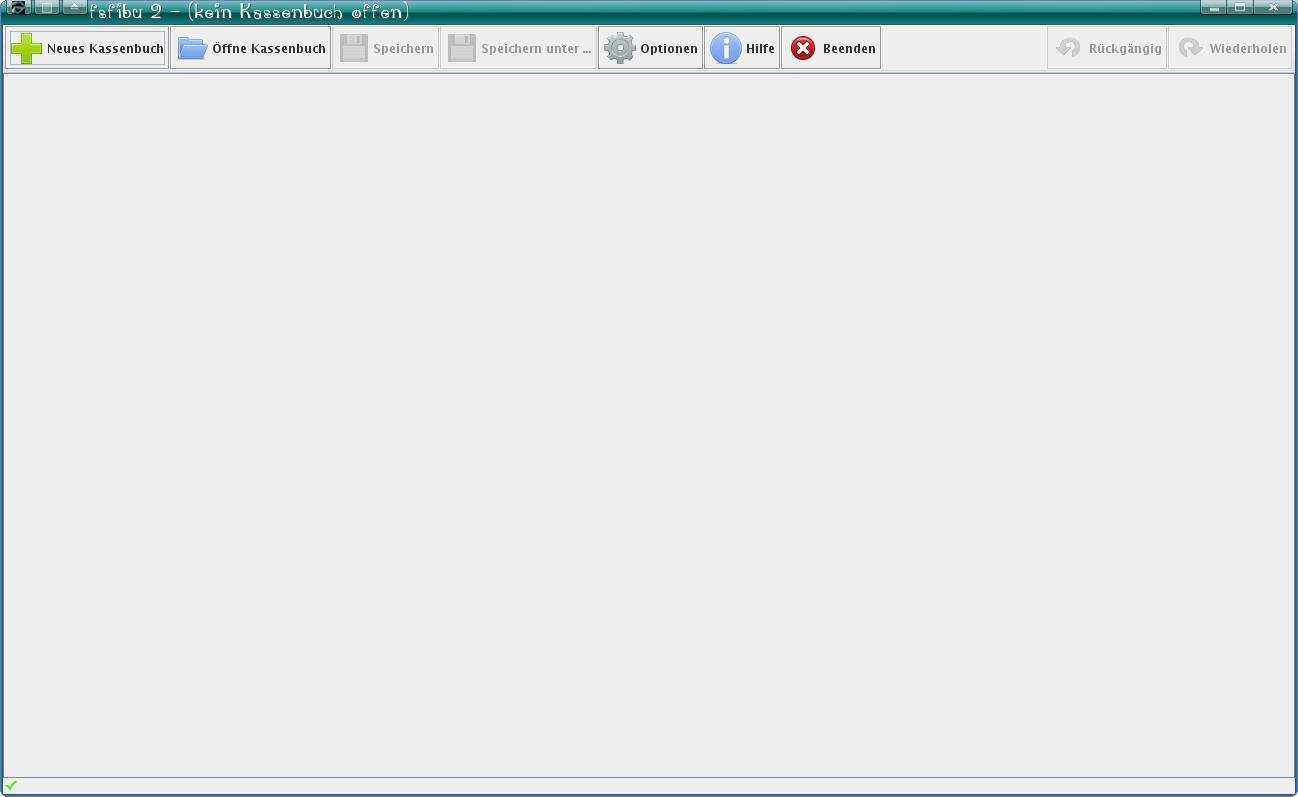
\includegraphics[width=10cm]{emptyprogram.jpg} 
\end{figure}
Wenn du fsfibu 2 das erste Mal öffnest, wird es ungefähr so aussehen: Nämlich leer. Am oberen Rand befindet sich das Hauptmenü. Es beinhaltet folgende Funktionen:
\begin{itemize}
 \item Neues Kassenbuch: Erstellt ein neues, leeres Kassenbuch und öffnet es
 \item Kassenbuch öffnet: Öffnet einen Dialog, um eine existierende Kassenbuchdate zu auszuwählen, die dann geladen wird
 \item Speichern: Speichert das aktuell ausgewählte Kassenbuch. Ist das Kassenbuch noch mit keiner Datei verknüpft, so wird ein entsprechende Dialog geöffnet. Kann mit Strg-S ausgelöst werden.
 \item Speichern unter: Speichert das Kassenbuch in einer anderen Datei
 \item Optionen: Hier kann man verschiedene Einstellungen am Programm vornehmen: Zur Zeit ist das lediglich die Sprache
 \item Hilfe: Dieser Knopf öffnet dieses Handbuch, sofern Java die entsprechende Programmzuweisung für pdf-Dokumente kennt. Wenn nicht, muss man das Handbuch eben 'von Hand' öffnen.
 \item Beenden: Schließt das Programm. Liegen noch ungespeicherte Änderungen vor, wird der Benutzer sicherheitshalber gefragt, ob er diese speichern möchte
 \item Rückgängig und Wiederholen: Hiermit werden Änderungen am derzeit ausgewählten Kassenbuch rückgängig gemacht oder wiederholt.
\end{itemize}

fsfibu 2 kann beliebig viele Kassenbücher gleichzeitig öffnen. Für jedes Kassenbuch wird dann ein neuer Tab angelegt. Beim Beenden merkt sich das Programm, welche Kassenbücher zuletzt offen waren und öffnet sie beim nächsten Start automatisch.

\subsection{Dateiformate}
fsfibu 2 Kassenbücher werden im XML-Format gespeichert. Das Programm kann 'erraten', ob eine XML Datei ein Kassenbuch enthält (ebenso wie es erraten kann, ob diese Datei ein altes, mit fsfibu 1 kompatibles Kassenbuch enthält) und wird den Benutzer warnen, falls es der Meinung ist, dass es sich um ein Fremdformat handelt. Es sollte generell nie in der XML-Datei selbst etwas geändert werden, da so u.U. beim nächsten Laden Daten verloren gehen.

\subsection{Sprache}
fsfibu 2 kann in verschiedenen Sprachen dargestellt werden. Die zu Verfügung stehenden Sprachen findet man unter 'Optionen' im Hauptmenü. Eine entsprechende Änderung wird aber erst nach einem Neustart des Programms wirksam. Siehe auch \ref{language}.

\section{Die Module}
\begin{figure}[h!]
 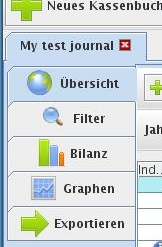
\includegraphics{modules}
\end{figure}

Wenn man ein Kassenbuch öffnet, sieht man links eine weitere, vertikale Liste von Tabs. Jedes dieser Tabs steht für ein Modul, d.h. einen Teil von fsfibu 2, der eine bestimmte Aufgabe erfüllt. Wir werden diese Module im Folgenden alle durchgehen. Anzumerken ist noch, dass das Programm sich bei Beenden die meisten der vorgenommenen Einstellungen in jedem Modul merkt (bspw. welche Filteransichten offen sind, etc...) und sie beim nächsten Start wiederherstellt.

\subsection{Übersicht}
Die Übersicht beinhaltet eine Komplettübersicht über das Kassenbuch in Form einer Tabelle aller Einträge. Des weiteren stehen in einer Werkzeugleiste noch mehrere Optionen zur Verfügung und ganz unten wird eine kurze Bilanz der Tabelle angezeigt.

\subsubsection{Die Tabelle}
Die Tabelle enthält Messpunkte, bzw. Jahrestrenner (blau unterlegt) und Einträge (weiß unterlegt). Messpunkte und Jahrestrenner dienen dazu, Einträge sichtbar voneinander zu trennen und Zwischenbilanzen anzuzeigen. Dabei sind Jahrestrenner nichts anderes als Messpunkte zum 31.12. eines Jahres. In der ersten Spalte der Tabelle wird zu jedem Eintrag angezeigt, ob zusätzliche Anmerkungen vorgenommen wurden und ob Informationen zu diesem Eintrag fehlen. Bewegt man dann die Maus über das Feld in der ersten Spalte, wird eine Zusammenfassung des Fehlers angezeigt. Weitere Informationen erhält man, wenn man die Maus über das Wert- oder Kto.-Informationen-Feld bewegt. Im ersten Fall wird eine Zwischenbilanz bis zu diesem Eintrag (einschließlich) angezeigt, im zweiten Fall eine übersichtlichere Zusammenfassung (mit Zuordnung der einzelnen Informationen). 

\subsubsection{Einträge erstellen / editieren}
Ein Eintrag besteht aus folgenden Informationen:
\begin{itemize}
 \item Name: Ein beschreibender Name. Darf nicht leer sein
 \item Datum: Das Datum des Eintrags, normalerweise ein Rechnungsdatum o.ä.
 \item Wert: Der Wert des Eintrags in Euro
 \item Kategorie: Jeder Eintrag liegt in einer Kategorie. Eine Kategorie ist dabei schlussendlich nichts anderes als eine Sequenz von Zeichenketten. Jede Zeichenkette steht dabei für eine weitere Spezialisierung, bspw. 'Lebewesen'-'Säugetiere'-'Hund'. Man kann eine Kategorie entweder aus den bereits bestehenden wählen, zu einer gewählten Kategorie eine neue Unterkategorie erstellen oder eine komplett neue Kategorie kreiieren.
 \item Konto: Jeder Eintrag repräsentiert eine Bewegung auf einem Konto. Das muss aber kein Bankkonto sein, sonder kann auch eine Handgeldkasse o.ä. sein.
 \item Konteninformationen: Zu jedem Konto gehören bestimmte zusätzliche Informationen, die man angeben kann (oder sollte). Je nachdem, welches Konto man gewählt hat, kann man Werte zu diesen Feldern hier eingeben.
 \item Zusätzliche Anmerkungen: Manchmal erfordert ein Eintrag zusätzliche klärende Anmerkungen. Die können hier eingetragen werden, sofern das entsprechende Häkchen gesetzt ist
\end{itemize}
\textbf{Hinweis zum Editieren:} Im ganzen Programm gilt: Ist ein eingetragener Wert in irgendeiner Form ungültig oder kritisch, wird neben dem Textfeld ein Warnzeichen angezeigt. Bewegt man die Maus darüber, erhält man eine Erklärung darüber, wo der Fehler liegt.

\subsubsection{Die Werkzeugleiste}
Die Werkzeugleiste bietet folgende Optionen:
\begin{itemize}
 \item Neuer Eintrag / Editieren / Löschen: Die drei ersten Knöpfe dienen dazu, Einträge neu zu erstellen, zu bearbeiten oder zu löschen. Dabei können beliebig viele Einträge auf einmal bearbeitet oder gelöscht werden.
 Ein neuer Eintrag kann auch mit Strg-N erstellt werden und ein existierender mit 'Entf' gelöscht werden.
 \item Drucken: Das Kassenbuch kann als einfache Tabelle sofort gedruckt werden. Die Messpunkte und Jahrestrenner werden dabei ausgelassen. Im entsprechenden Druckdialog kann man angeben, welcher Titel über der Tabelle erscheinen soll, in welcher Schriftgröße gedruckt werden soll und ob die Anmerkungen ebenfalls gedruckt werden sollen. Ein Eintrag kann auch durch Doppelklick editiert werden.
 \item Als csv exportieren: Analog zum CSV Tabellenformat werden hier allerdings nur die sichtbaren Einträge exportiert.
 \item Editiere Messpunkte: Hiermit öffnet sich ein Dialog zum Editieren der Messpunkte. Ein Messpunkt besteht aus einem Namen und einem Datum, das angibt welche Einträge vor ihm liegen (nämlich alle bis einschließlich zu diesem Datum).
 \item Jahrestrenner und Messpunkte ein/ausschalten: Hiermit werden die Jahrestrenner und Messpunkte aus der Tabelle entfernt oder wieder hinzugefügt. Ist ein Messpunkt sichtbar, wird in dieser Zeile eine Zwischenbilanz vom letzten Messpunkt bis zu diesem angezeigt.
 \item Jahr und Kategorie wählen: In der Übersicht kann bereits beschränkt gefiltert werden. Hier kann man auswählen, aus welchem Jahr und welcher Kategorie man Einträge sehen möchte.
 \item Namen und Beschreibung bearbeiten: Zu jedem Kassenbuch gehört ein Name (der dann im Tab des Kassenbuchs steht) und eine Beschreibung. Diese können hier editiert werden.  
 \item Kontostartwerte bearbeiten: Zu jedem Konto, dass im Kassenbuch verwendet wird, gehört ein Startwert. Das ist die Menge an Geld, die zu Beginn der Buchführung in diesem Kassenbuch auf dem Konto lag. Der Knopf lässt eine Tabelle erscheinen, in der die entsprechenden Werte editiert werden können.
\end{itemize}

\subsubsection{Die Bilanz}
Am unteren Bildrand wird eine grobe Bilanzübersicht angezeigt. Hier kann man grundsätzlich erst mal wählen, ob man eine Bilanz über die gesamte Tabelle möchte oder nur über einen Teil, der durch die derzeitige Auswahl bestimmt ist. Hat man einen Teil der Tabelle ausgewählt, wird neben 'Auswahl:' angezeigt, welcher Teil dann bilanziert wird.
Bilanziert man über alles, kann man dann nochmal wählen, ob man nur zwischen bestimmten Messpunkten bilanzieren möchte.	Daneben wird dann eine Bilanz der Konten angezeigt, d.h. ihr Kontostand vorher, nachher und die entsprechende Differenz. Dabei bedeutet 'Vorher': Die Summer aller Einträge vor dem ersten bilanzierten Eintrag und 'Nachher' ist eben diese Summer plus alle bilanzierten Einträge.

Ganz rechts sieht man dann noch eine Gesamtsumme für jede Kategorie und die Gesamtsumme über alle bilanzierten Einträge.

\subsection{Filter}
Die Filtersicht besteht aus prinzip aus mehreren Übersichten, nach Tabs getrennt. Der obere Teil der Werkzeugleiste, die Tabelle und die Bilanz sind im Prinzip identisch. Zu jeder Filtersicht gehört aber noch ein Filter, mit dem sich deutlich feiner nach bestimmten Einträgen suchen lässt.

Zuerst einmal erstellt man eine neue Filtersicht, in dem man auf 'Neu' klickt. Jede neue Filtersicht hat erst mal einen leeren Filter, lässt also alle Einträge zu. Um einen Filter zu editieren, klickt man auf das Lupensymbol rechts oben und macht den Filtereditor somit sichtbar. 

Statt einen neuen Filter zu kreiieren, kann man auch einen in einem anderen Modul erstellten Filter kopieren. Dazu wählt man aus der Liste neben 'Kopie' den entsprechenden Filter aus.

\subsubsection{Tabtitel}
Bei der Erstellung eines neuen Tabs kann man sofort dessen Titel editieren. Das Bearbeiten kann man jederzeit mit Enter beenden oder mit Esc abbrechen. Will man den Titel im Nachhinein editieren, muss man einfach doppelt darauf klicken.

\subsubsection{Der Filtereditor}
\begin{figure}[h]
 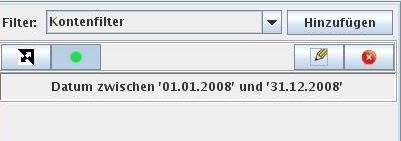
\includegraphics{filtereditor1}
\end{figure}
Jeder Filter besteht schlussendlich aus einer Liste (oder einem Stapel) verschiedener spezieller Filter. Im Filtereditor ist ganz oben eine Klappliste zu sehen, aus der man die Art von speziellem Filter wählen kann, die man hinzufügen möchte. 
Hat man einen Filter hinzugefügt, erscheint am unteren Ende des Stapels ein Kästchen, das am oberen Rand eine Reihe von Symbolen enthält:
\begin{itemize}
 \item Negieren: Hiermit lässt sich der Effekt des Filters ins Gegenteil verkehren
 \item Ein/Ausschalten: Manchmal möchte man einen Filter außer Kraft setzen, ohne ihn gleich zu löschen (Es ist vielleicht ein sehr komplizierter Filter). Das kann man mit diesem Knopf tun
 \item Übernehmen / Abbrechen: Wenn man einen Filter neu hinzufügt, befindet er sich sofort im Editiermodus. Mit diesen beiden Knöpfen kann man seine Änderungen übernehmen oder verwerfen. Danach werden diese beiden Knöpfe durch einen mit einem Bleistiftsymbol ersetzt, durch den man wieder in den Editiermodus gelangt. 
 \item Löschen: Mit dem letzten Knopf wird der Filter aus dem Stapel entfernt.
\end{itemize}
Bevor einige Filter im Einzelnen durchgesprochen werden, möchte ich einige Dinge besprechen, die häufig ähnlich konfiguriert werden. Es gibt bei fast allen Filtern die Wahlmöglichkeit zwischen 'Gleichheit', 'Regulärer Ausdruck' und 'Bereich'. Man kann hier also wählen, ob nach Einträgen gesucht werden soll, bei denen ein bestimmter Wert genau gleich einem Vergleichswert ist, auf einen regulären Ausdruck passt oder in einem bestimmten Bereich liegt. Bei den Bereichsfiltern gilt stets: Lässt man das Feld leer, bedeutet das, dass keine untere/obere Grenze gewünscht ist. Bereich bedeutet im Fall von Text, dass ein Text alphabetisch zwischen Min und Max liegen muss.

\subsubsection{Konteninformationsfilter}
Einen Konteninformationsfilter legt man für ein bestimmtes Feld an, beispielsweise der Rechnungsnummer, das man aus einer Liste auswählt. Danach filtert man wie oben beschrieben. Für Felder, die stets numerische Werte enthalten, wie z.B. Kontoauszug, kann man angeben, dass Bereichswerte explizit als numerische Werte interpretiert werden sollen, statt als Text.

\subsubsection{Kategorienfilter} 
Beim Kategorienfilter kann man entweder nach genau einer Kategorie filtern (Man wählt sie aus), oder auf einer bestimmten Ebene nach verschiedenen Kriterien filtern. Dabei bezeichnet 1 die erste Ebene, d.h. bei 'Lebewesen'-'Säugetiere'-'Hunde' wäre Ebene 3 eben 'Hunde'.

\subsubsection{Kontenfilter}
Beim Kontenfilter kann man sich aussuchen, ob man entweder nur Einträge eines bestimmten Kontos möchte oder entsprechen der Zeichenkette, die das Konto repräsentiert, feiner filtern möchte. So würde Regulärer Ausdruck: B.* beispielsweise nach Einträgen suchen, deren Konto mit einem B beginnt.

\subsection{Bilanz}
In der Bilanzansicht wird eine Bilanz - nach Einnahmen, Ausgaben getrennt - einer bestimmten Untermenge von Einträgen angezeigt. Welche Einträge das sind, bestimmt ein Filter, der genauso wie in der Filteransicht konfiguriert wird. Die Bilanzansicht ist eine Baumansicht, die der Hierarchie der Kategorien entspricht. Rechts in der Tabelle steht dann die entsprechende Bilanz der gesamten Kategorie (d.h. inklusive Unterkategorien). Gibt es Einträge in einer Kategorie, die auch noch Unterkategorien hat, so werden diese Einträge in einem Unterknoten der Kategorie bilanziert, der den gleichen Namen - allerdings in Klammern - trägt.

Da man eine solche Bilanz auch drucken kann, kann man rechts in der Tabelle noch weitere Einstellungen vornehmen:
\begin{itemize}
 \item Unsichtbar machen: Eine Kategorie kann unsichtbar gemacht werden, wenn man sie kurzzeitig rausrechnen möchte und/oder in der Bilanz nicht sehen will
 \item Maskieren: Eine Kategorie kann maskiert, d.h. in der Druckversion unter anderem Namen dargstellt werden.
\end{itemize}

Mit den beiden vorhanden Knöpfen kann eine Bilanz gedruckt (Analog zum Druck des Kassenbuchs) oder als csv exportiert werden, wobei die csv-Datei einer Tabelle entspricht, die wie die voll ausgeklappte Tabelle der Bilanz aussieht, aber inklusive Unsichtbarkeiten und Maskierungen.

Es gibt einen weiteren Knopf (``Kuchendiagramm anzeigen''), der ein neues Fenster öffnet, in dem eine Kuchenansicht der Einnahmen oder Ausgaben der Bilanz angezeigt wird. Hier kann man zwischen Einnahmen und Ausgaben wechseln, sich nur eine bestimmte Kategorie anzeigen lassen, oder auswählen, ob nur direkte Unterkategorien oder nur die niedrigsten Kategorien verwendet werden.

\subsection{Graphen}
Auch die Graphenansicht wird durch Filter konfiguriert, genau wie die beiden Module zuvor. Sie stellt für die ausgewählten Eintrag einen Zeitreihengraph dar. Zusätzlich dazu kann ein gleitender Mittelwert über einen bestimmten Zeitraum von Tagen eingezeichnet werden. Man kann in den Graph hineinzoomen, in dem man ein entsprechendes Rechteck mit der Maus zieht. Herauszoomen und andere Optionen sind im Kontextmenü verfügbar, das man mit der rechten Maustaste öffnet.

\textbf{Hinweis:}Der eigentliche Graph wurde nicht von mir implementiert, sondern stammt aus der Bibliothek JFreeChart, siehe auch www.jfree.org/jfreechart/. Des Weiteren ist diese Ansicht u.U. recht langsam, d.h. es dauert recht lange, bis der Graph dargstellt wird.

\subsection{Exportieren}
Das Exportmodul stellt keine Daten des Kassenbuchs dar, sondern dient dazu, es in verschiedene Formate zu exportieren, sowie regelmäßige Backups zu konfigurieren. Dazu wählt man zuerst das gewünschte Format aus. Will man das Kassenbuch nur einmalig exportieren, klickt man auf 'Exportieren' und wählt eine Datei zum Speichern aus. Will man dagegen ein regelmäßiges Backup einrichten, wählt man 'Regelmäßige Sicherung', ein Sicherungsintervall in Minuten und die Datei, in die das Backup gespeichert wird. 

Die von Anfang an verfügbaren Standardformate sind:
\subsubsection{Fsfibu 2 format}
Das ist das Format, in dem Kassenbücher standardmäßig gespeichert werden. Ein Export macht hier natürlich wenig Sinn, dieses Format dient hauptsätzlich zur regelmäßigen Sicherung
\subsubsection{Fsfibu 1 format}
Das Format der ersten Version von fsfibu 1 unterscheidet sich erheblich vom neuen Format und ist nicht so ohne Weiteres kompatibel. Trotzdem ist (unter möglichem Verlust von Informationen) ein Import/Export möglich. Dabei gilt:
\begin{itemize}
 \item Nur Startwerte für Bankkonto und Kasse werden übernommen
 \item Alle Messpunkte werden übernommen
 \item Name, Wert, Datum und Anmerkungen eines Eintrags werden übernommen
 \item Das 'Echtdatum'-Feld des konvertierten Eintrags beinhaltet das Datum des Eintrags
 \item Nur die ersten beiden Ebenen einer Kategorie werden als 'Kategorie' und 'Gruppe' übernommen
 \item Jeder Eintrag, der nicht zu Bankkonto oder Kasse gehört, geht verloren
 \item Die Kontoinformationen zu Bankkonto und Kasse werden übernommen
\end{itemize}
\subsubsection{CSV Tabellenformat}
Um das Kassenbuch in Tabellenform in ein Tabellenkalkulationsprogramm zu importieren, eignet sich hervorragen das Format csv (comma-separated value). Hier werden Daten lediglich als Text gespeichert, der von Excel oder OpenOffice als Tabelle interpretiert wird. Dabei zeigt ein Zeilenumbruch die nächste Zeile an und ein bestimmtes Trennsymbol die nächste Spalte. Das Trennsymbol bei allen fsfibu 2 Exporten ist aus technischen Gründen das Semikolon, nicht das Komma.

Das CSV Tabellenformat exportiert das Kassenbuch als einfache Tabelle, wie sie auch in der Übersicht zu sehen ist (allerdings wird die Indikatorspalte vorne weggelassen).
\subsubsection{CSV OpenOffice Format}
Vor fsfibu 1 wurde unser Kassenbuch in einer Tabelle in OpenOffice verwaltet. Dieses CSV-Format speichert das Kassenbuch in einer Form, die mit dieser Tabelle kompatibel ist.


\chapter{Erweiterungen}

fsfibu 2 ist von vornherein so geschrieben worden, dass sich mehrere Aspekte leicht erweitern lassen. 'Leicht' bedeutet in diesem Zusammenhang allerdings noch immer, dass man, um eine Erweiterung selbst zu erstellen, durchaus Java programmieren muss. Man braucht allerdings nicht jedes Mal den Quellcode des ganzen Projekts zu beschaffen und zu kompilieren. Trotz allem ist dieses Kapitel relativ technisch und ohne gewisse Grundkenntnisse in Java wahrscheinlich völlig uninteressant.

Das Erweiterungskonzept funktioniert eigentlich immer auf die gleiche Weise: Man schreibt eine Klasse, die eine Erweiterung in einem bestimmten Bereich darstellen soll (beispielsweise einen Filter) und kopiert die .class - Datei, die beim Kompilieren entstand, in den zugehörigen Ordner im Hauptverzeichnis von fsfibu 2(in diesem Fall eben /filters). Beim nächsten Programmstart wird die Erweiterung automatisch geladen. Des Weiteren muss eine solche Klasse immer eine Methode implementieren, die eine eindeutige ID zurückgibt. Für jeden Typ von Erweiterungen gibt es eine entsprechende Konvention für diese ID, die zumindest von mir eingehalten wurde. Indem man sich also NICHT daran hält, geht man relativ sicher, nicht mit den von mir gewählten IDs zu kollidieren.

\textbf{Hinweis:} Damit eine Erweiterung erkannt wird, ist immer ein Neustart des Programms notwendig.

\section{Module}
Die mächtigste und flexibelste Erweiterungsmöglichkeit stellen die Module dar. Ein Modul entspricht schlussendlich einem Tab links im fsfibu 2 Hauptfenster. Für jedes registrierte Modul kreiiert das Programm beim Laden eines Kassenbuchs automatisch einen Tab. Eine Modulklasse muss im Paket \textit{fs.fibu2.module} liegen und das Interface \textit{fs.fibu2.view.render.JournalModule} implementieren. Die entsprechende Datei gehört ins Verzeichnis modules/. Dieses Interface stellt neben dem Text und dem Icon für den Reiter auch eine Methode zur Verfügung, über die das Programm die eigentliche grafische Modulkomponente erhält. Die erstellte Klassendatei des Moduls kommt in das Verzeichnis (fsfibu2)/modules. Die Konvention für die ID eines Moduls lautet \textit{ff2module\_} + ein beschreibender Text, bspw. \textit{ff2module\_bilancial}.

\section{Filter}
Kassenbucheinträge können nach praktisch jeder ihrer Eigenschaften gefiltert werden. Trotzdem erhebt fsfibu 2 natürlich keinen Anspruch auf Vollständigkeit. Deshalb können problemlos weitere Filter hinzugefügt werden. Man schreibt einfach eine Klasse, die im Paket \textit{fs.fibu2.filter} liegt und das Interface \textit{fs.fibu2.filter.EntryFilter} implementiert. Die entsprechende Klassendatei kommt dann in das Verzeichnis (fsfibu2)/filters. Der neue Filter wird vom Program automatisch in die Liste der verfügbaren Filter im Filtereditor eingefügt. 

Neben den eigentlichen Filtermethoden muss eine solche Klasse noch eine Methode implementieren, die eine Editorkomponente zurückgibt. Diese Editorkomponente muss dann die Klasse \textit{fs.fibu2.filter.EntryFilterEditor} beerben. Soll der Filter nicht editierbar sein (bspw. weil er auch gar keine variablen Parameter hat), sollte die Methode einfach \textit{null} zurückgeben.

Die ID-Konvention für Filter lautet \textit{ff2filter\_} + irgendwas.

\section{Konten}
fsfibu 2 unterstützt von Haus aus zwei Kontentypen: Bankkonto und Kasse. Das liegt daran, dass das genau die beiden Kontentypen waren, die wir in der Fachschaft benötigten. Das wird natürlich nicht für jeden Zweck ausreichen. Deshalb gibt es die Möglichkeit, sich eigene Kontoklassen zu schreiben. Die entsprechende Klasse muss im Paket \textit{fs.fibu2.account} liegen und das Interface \textit{fs.fibu2.data.model.Account} implementieren. Eine neue Klasse wird automatisch in die Liste der möglichen Konten im Eintragseditor hinzugefügt. Die Klassendatei gehört in das Verzeichnis accounts/.

Die ID-Konvention für Konten ist, den Namen des Kontos klein zu schreiben und Leerzeichen durch Unterstriche zu ersetzen, also bspw. \textit{cash\_box}

\section{Export}
Man kann ein Kassenbuch in mehrere verschiedene Formate exportieren. Unter Umständen benötigt man aber ein sehr bestimmtes Format. Den entsprechenden Exporter kann man sich dann selbst schreiben. Er muss das Interface \textit{fs.fibu2.data.format.JournalExport} implementieren. Export unter fsfibu 2 unterstützt keine variablen Parameter, wie z.B. Filter oder ähnliches. Die Exportmethode enthält als Argumente lediglich das zu exportierende Kassenbuch und den Namen der Datei, in die es exportiert werden soll. Die Klassendatei gehört in das Verzeichnis exports/.

\section{Bibliotheken}
Ein aufwändiges Plugin, insbesondere ein neues Modul, braucht unter Umständen weitere, selbst definierte Klassen. Würde man nur die Klassendatei des Moduls laden, käme man nicht weit, der ClassLoader würde all diese Klassen nicht kennen. Deswegen gibt es die Möglichkeit, eigene jar - Bibliotheken beim Programmstart zu laden. Die Datei muss auf .jar enden und im Verzeichnis pluginlibs/ liegen. Das Programm wird dann versuchen, sie vor den Plugins zu laden.

\section{Sprache}\label{language}
fsfibu 2 ist so gestaltet, dass es ohne größeren Aufwand in mehreren Sprachen dargstellt werden kann. Dazu wird eine Texttabelle im XML-Format verwendet, die alle in fsfibu 2 erscheindenen Texte in eben diesen Sprachen enthält. Die Tabelle kann mit dem von mir geschriebenen Programm POLYGLOT bearbeitet werden (das zum Paket fsframework gehört, bzw. unter /fsframework mit polyglot.jar gestartet werden kann). Die alte Tabelle muss allerdings nicht unbedingt durch eine neue ersetzt werden, es reicht auch, die neue, modifizierte Version unter anderem Namen in das Unterverzeichnis lang/. fsfibu 2 wird sie dann automatisch laden und als Update integrieren.

\end{document}
